%   Filename    : chapter_4.tex 
\chapter{Research Methodology}
This chapter lists and discusses the specific steps and activities that will be performed  to accomplish the project. 
The discussion covers the activities from pre-proposal to Final SP Writing.

\section{Research Activities}
\subsection{Development Framework}
The proposed application is an interconnected and interdependent system, such that one feature is either dependent on or a prerequisite of another (i.e. the registration feature is required before the reporting and verification feature; the main-companion app binding feature requires that the main and companion app interfaces have been built).
\\\\Due to this reason, the researchers will adopt a modified version of the Feature-Driven Development (FDD) agile framework. FDD approaches software development by developing an overall model, listing all features (and how they interact), planning each feature, then focusing on designing and building one feature at a time \cite{productplan2022}. This modified version of FDD will include feature documentation after each feature is built and integrated, and the system prototype will be released only when all features have been built, integrated, and tested.
\\\\As seen in Figure \ref{fig:FDDFramework}, the system will be developed by first developing the entire model, list all the features, plan the other by which to develop the features so that they can be integrated.

\begin{figure}[!h]
    \centering
    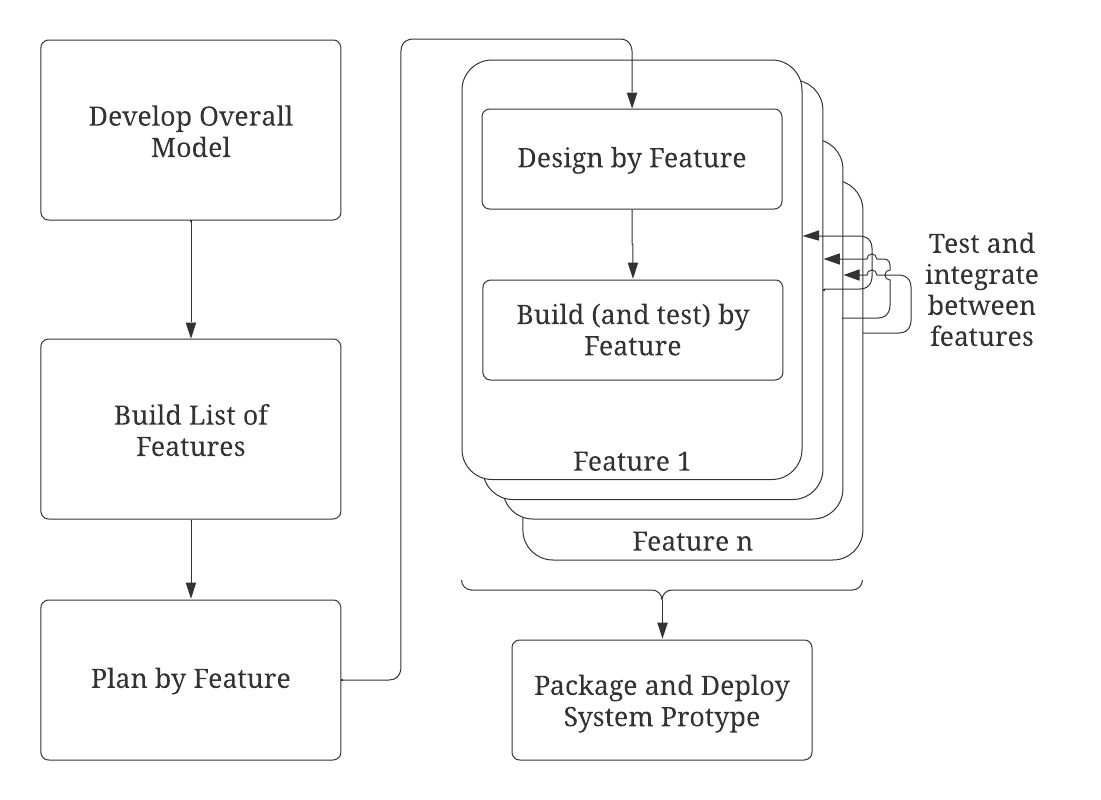
\includegraphics[width=\textwidth]{Chapter3/Chapt3_DevFramework.jpeg}
    \caption{Modified Feature-Driven Development (FDD) Framework}
    \label{fig:FDDFramework}
\end{figure}

\subsection{Calendar of Activities}

A Gantt chart showing the schedule of the activities should be included as a table. For example:

Figure \ref{fig:timetableactivities} shows the Gantt Chart of all activities to be undertaken from the conception, to the development, and the analysis of the proposed application. Since the development framework used is FDD, development is scheduled by each feature.

\begin{figure}[!h]
    \centering
    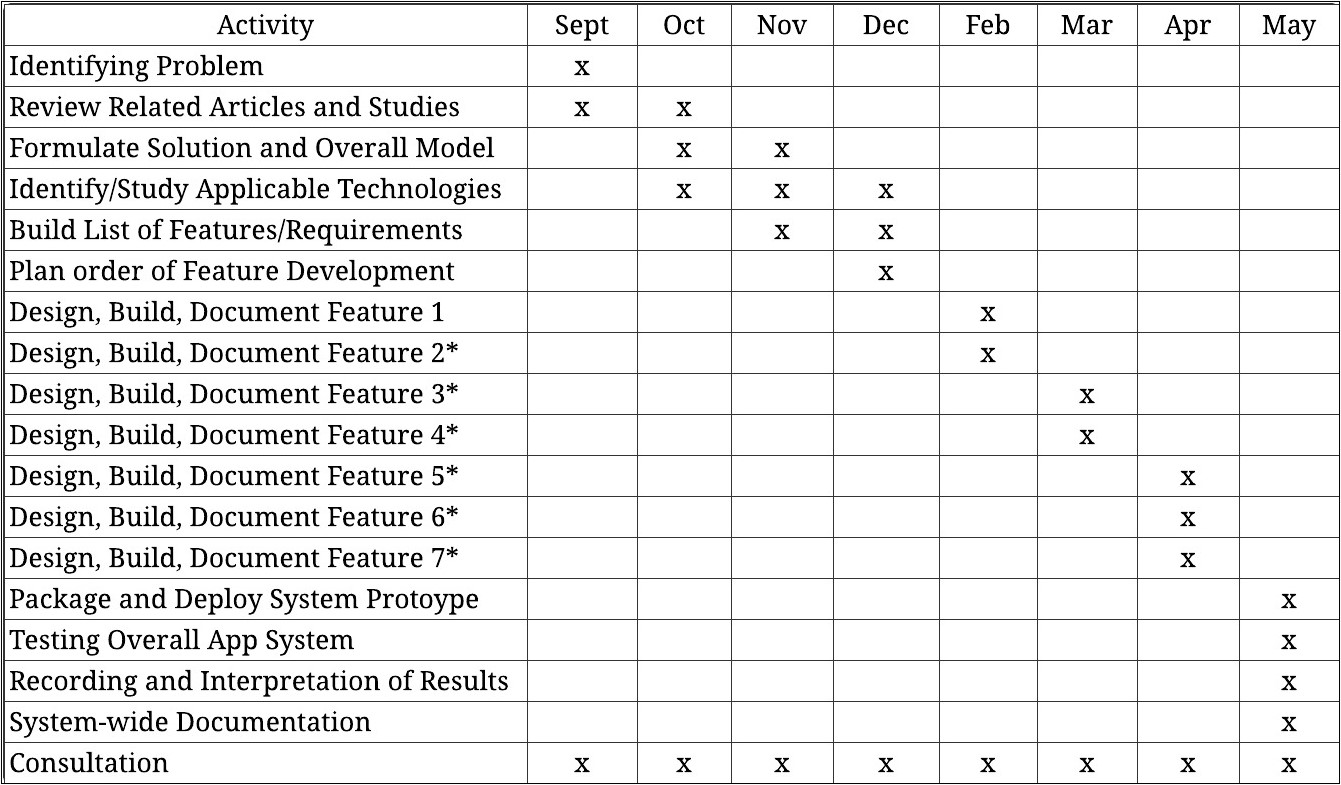
\includegraphics[width=\textwidth]{figures/Chapter3/Chapt3_calendar.jpg}
    \caption{Timetable of Activities}
    \label{fig:timetableactivities}
\end{figure}

The order of the features to be developed as per the table are as follows :
\begin{itemize}
    \item Feature 1 - Firebase serverless database backend
    \item Feature 2 - main app registration system
    \item Feature 3 - main app reporting and PNP Admin App verification feature
    \item Feature 4 - main app location-based notification feature for nearby PNP-verified reports
    \item Feature 5 - companion app and its ``Find Me" feature
    \item Feature 6 - main-companion apps binding
    \item Feature 7 - main app ``Find Companion" feature
\end{itemize}

\section{Development Tools}
\subsection{Software}

\subsubsection{Github}
GitHub is a web-based tool that utilizes Git, an open source version control that enables several users to make distinct modifications to applications or software simultaneously \cite{digitalGovGitHub}. GitHub is currently being used by over 94 million software developers, 4 million plus organizations, and has created over 330 million repositories for varied software \cite{github}.

\subsubsection{Visual Studio Code}
Visual Studio Code is a compact yet capable source code editor for macOS, Windows, and Linux that runs on your desktop. It supports multiple programming and scripting languages like JavaScript, TypeScript, and Node.js, as well as a robust ecosystem of extensions for additional languages and runtimes (including C++, C\#, Java, Python, PHP, Go, and.NET) \cite{microsoft_2021}.

\subsubsection{Android Studio}
Android Studio is the official Integrated Development Environment (IDE) for developing Android mobile apps. It is based on the IntelliJ IDEA development tools and code editor. When compared to other IDEs, Android Studio is considered hefty; however, this is expected considering that it incorporates various integrations and add-ons like a flexible Gradle-based build system, built-in emulators, code templates, extensive testing tools, and many others to guarantee that development is as interactive and fluid as possible \cite{androidStudio}.

\subsubsection{Flutter}
Flutter is a Google open-source framework used for creating attractive, locally built, multi-platform apps out of a single codebase. For rapid efficiency and performance on any device, Flutter code compiles to ARM or Intel machine code, as well as JavaScript. Dart, a programming language designed for speedy programs on any platform, powers it \cite{flutter}. As the developers are aiming to deploy the proposed application on both the mobile (Android) platform for the main users and their companions, and on the Windows (desktop)  platform for the side of PNP, Flutter is an outstanding choice out of all the available frameworks and languages.

\subsubsection{Google Firebase}
As Firebase has a variety of products and services that it provides, such as Firebase Cloud Messaging (FCM) for messages as well as notifications for Android, Web Applications, and iOS, Firebase Auth, which is a service that can authenticate users using only client-side code, Real-time Database, a NoSQL database service, and Firebase Storage, which is a file transfer service \cite{khawas2018application}, Firebase remains to be the most optimal choice for a serverless mobile application that may require the said services, such as with the proposed application.

\subsubsection{Google Maps}
Google Maps, one of the world’s most influential applications \cite{mehta2019google}, provides multiple location services needed in the proposed application. This includes the pinging of the location of the user of the companion app, or perhaps even the pinpointing and updating of the location where a verified missing person was last seen.

\subsection{Hardware}
\subsubsection{Android Phone}
An Android phone is a type of smartphone that is operating using the operating system developed by Google, Android.

\subsubsection{Laptop}
The proposed application will be developed on laptop computers with the minimum specifications of an 8th generation Intel Core i3 CPU, and 8GB of RAM.

\subsection{Application Programming Interfaces (APIs)}
\subsubsection{Geofencing API}
The geofencing API lets the developers construct perimeters, also known as geofences, that encircle regions of interest. When a device crosses a geofence, your app receives a notice, allowing you to deliver a beneficial experience when users are nearby \cite{geofencing}.

\subsubsection{Geocoding API}
The Geocoding API converts addresses directly into geographic coordinates, which may then be used to set markers on a map or position the map  \cite{geocoding}.

\subsubsection{Distance Matrix API}
The Distance Matrix API offers travel distances and times for a matrix of origins and destinations, with rows holding duration and distance values for each pair \cite{distanceMatrix}.

\subsubsection{Maps Embed API}
With the help of the Maps Embed API, developers may add a Street View panorama or interactive map to an application being developed through only using a straightforward HTTP request \cite{mapsEmbed}.

\subsubsection{Places API}
The Places API is a service that employs HTTP requests to return information about locations. This API defines places as establishments, physical sites, or important points of interest \cite{placesAPI}. This API will help the developers to pinpoint the location of the nearest and most logically sound police station, and hence local PNP admin accounts, based on the location of the reports of missing persons.

\section{Application Requirements}
\subsection{Backend Requirements}
Listed below are the proposed and overall structure of all connections and relationships among all data, interfaces, users, and the serverless service. It is important to note as well that since this is still just the proposed architecture, the finalized form of it, and especially how data will be organized within Firebase, can be changed during the actual development if the developers ever find a more practical approach to it.

\subsubsection{Serverless Architecture}

\begin{figure}[!h]
    \centering
    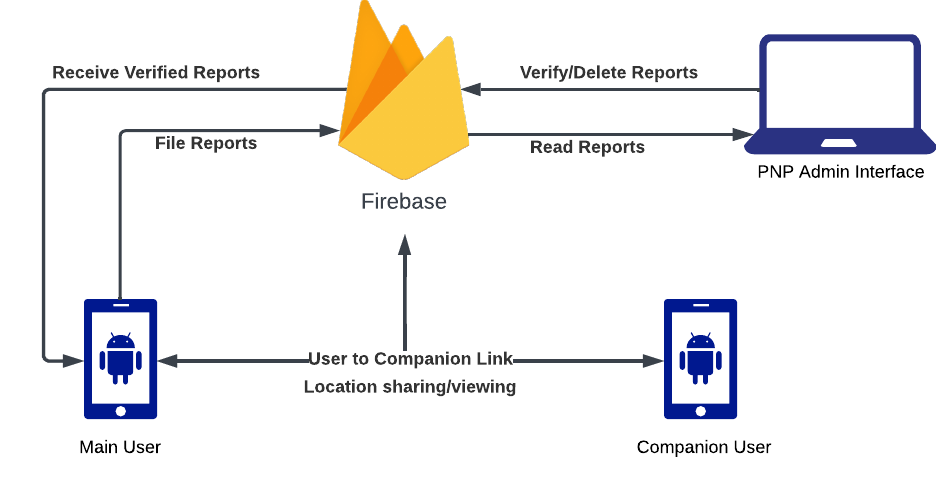
\includegraphics[width=\textwidth]{Chapter3/Chapt3_ServerlessArchitecture.png}
    \caption{Client-Serverless Architecture with Firebase}
    \label{fig:ServerlessFirebase}
\end{figure}

The overall serverless architecture of the proposed application and its system is portrayed in the diagram above. Firebase, as the serverless service being utilized, will be the storage of all data being utilized on all three interfaces. 

\subsubsection{Realtime Database structure for User, Companion, and PNP admin profiles}
Each profile type will be a node just under the root node as child nodes, namely, Main Users, Companions, and PNP Admins. 

\subsubsection{Realtime Database structure for sent reports}
As Firebase’s real-time database is structured as a tree, sent reports will be listed as child nodes of the user who sent them. This way, it will be easier to know who has filed what, and only the user who has filed an unverified report can directly see it. Once the PNP Admin interface has verified it, then that report will be displayed publicly.

\subsubsection{Images and other media storage}
The real-time database only functions on non-media data like text, integers, and location data; therefore, images used within the application interfaces (user image, missing person image) will be stored in Firebase’s cloud storage.

\subsection{User Interface Requirements}
\subsubsection{User (or Main) Interface}

\begin{figure}[!h]
    \centering
    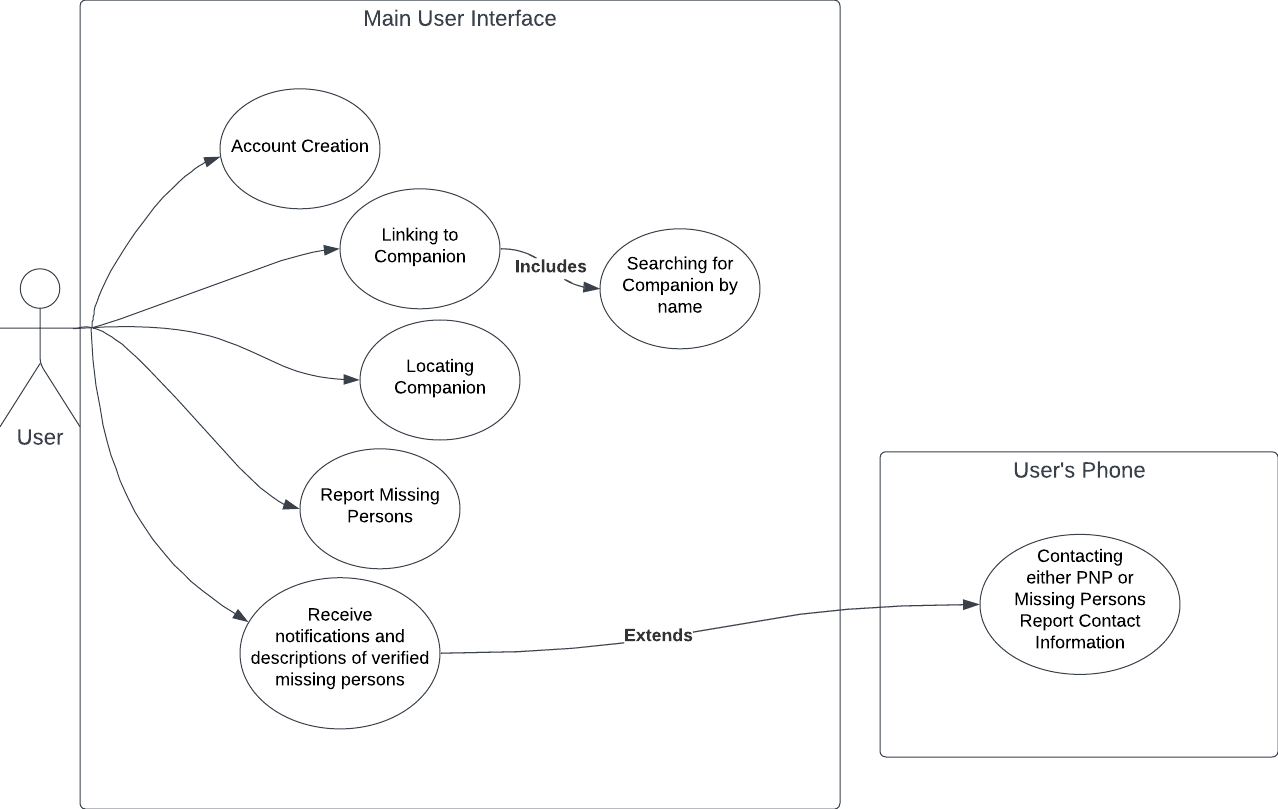
\includegraphics[width=\textwidth]{Chapter3/Chapt3_UseCase_Main.png}
    \caption{Use-Case Diagram for User (Main User Interface)}
    \label{fig:UseCaseMain}
\end{figure}
The User use-case diagram in Figure \ref{fig:UseCaseMain} illustrates all the possible tasks that a normal user could do within the application. User account creation will be done within the application itself, through Firebase auth’s authentication service using a registered email address and password. After the user has registered and confirmed his/her email address, his/her account will be created. Within the proposed application, the user can do a variety of things, one of which is linking to a companion PARGOM by searching him/her within the application’s search interface. 
\\\\When linked up to a companion PARGOM, the User can prompt to ask the latest tagged location of the said companion. A main feature within the application, also, is with the reporting of missing persons. This is done through the application by filling out a form with the details required for the missing persons report, which would then be filed towards the most logically sound police-station. Users can also receive notifications with regards to the descriptions and features of any missing persons report that have been verified by the PNP.

\subsubsection{Companion App Interface}

\begin{figure}[!h]
    \centering
    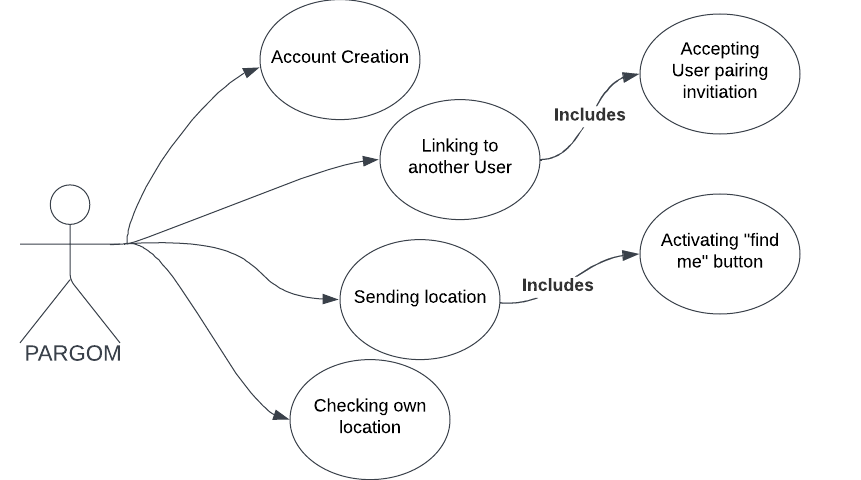
\includegraphics[width=\textwidth]{Chapter3/Chapt3_UseCase_PARGOM.png}
    \caption{Use-Case Diagram for PARGOMs (Companion Interface)}
    \label{fig:UseCasePARGOM}
\end{figure}
\\\\The use-case diagram for PARGOMs and the companion interface of the application is seen in Figure \ref{fig:UseCasePARGOM}. In principle, PARGOM user accounts are a miniaturized version of the base application. These user accounts are intended for users who are children, the elderly, or anyone else that can be considered as a person at risk of going missing. As such, every PARGOM, just like the User accounts, can also register the same way using Firebase auth authentication services. 
\\\\Being a companion account, as well, allows PARGOM account users to receive invitations to becoming a companion of any Users they deem to be trustworthy of their location, for example, a child companion/PARGOM account holder to his/her User account holder parent. PARGOM accounts can also activate a “find me” button in which he/she can share his/her location directly with the User account it is connected to. Lastly, PARGOM accounts users can also check their own location within the app.

\subsubsection{PNP Admin App Interface}

\begin{figure}[!h]
    \centering
    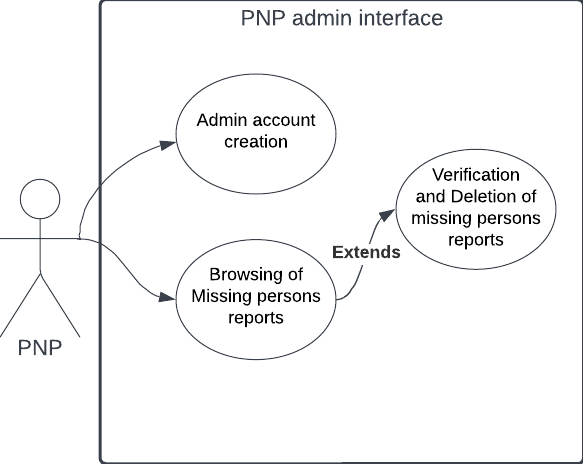
\includegraphics[width=\textwidth]{figures/Chapter3/Chapt3_UseCase_PNP.png}
    \caption{Use-Case Diagram for PNP (PNP Admin Interface)}
    \label{fig:UseCasePNP}
\end{figure}
\\\\The PNP and PNP Admin interface use-case diagram is shown in Figure \ref{fig:UseCasePNP}. The PNP admin accounts are created in a different manner compared to the previously stated accounts. First, PNP admin accounts cannot be created through the PNP admin interface (e.g., a ``Register" option) in order to control and limit the number of admin users within a police station to only one, who can only handle missing persons reports within their jurisdiction. 
\\\\Local police stations can request PNP admin accounts from the developers in order for it to be recognized as an ``admin" account rather than any main user or PARGOM companion account. Once a PNP admin has logged in to the PNP admin interface, he or she, as an official, can then browse and either verify or delete missing person reports filed within their jurisdiction.

\subsection{Functional Requirements}
\subsubsection{User Registration}
Main and Companion application Users should be able to launch their respective application interfaces and register through the log-in and registration page in-app. Once verified and registered, both user types can then utilize and log in into the application. 

\subsubsection{PNP Admin Account Creation}
PNP Admin accounts users should be able to contact the developers using the information displayed about logging in through the PNP Admin interface, in order for each PNP station to have a PNP Admin Account. 

\subsubsection{Reporting and Receiving Updates}
General users should be able to fill out and send the MP case report form via the main app interface to the PNP station that has jurisdiction of the area where the reported person went missing, and receive updates via the main app with regards to the status of the report.

\begin{figure}[!h]
    \centering
    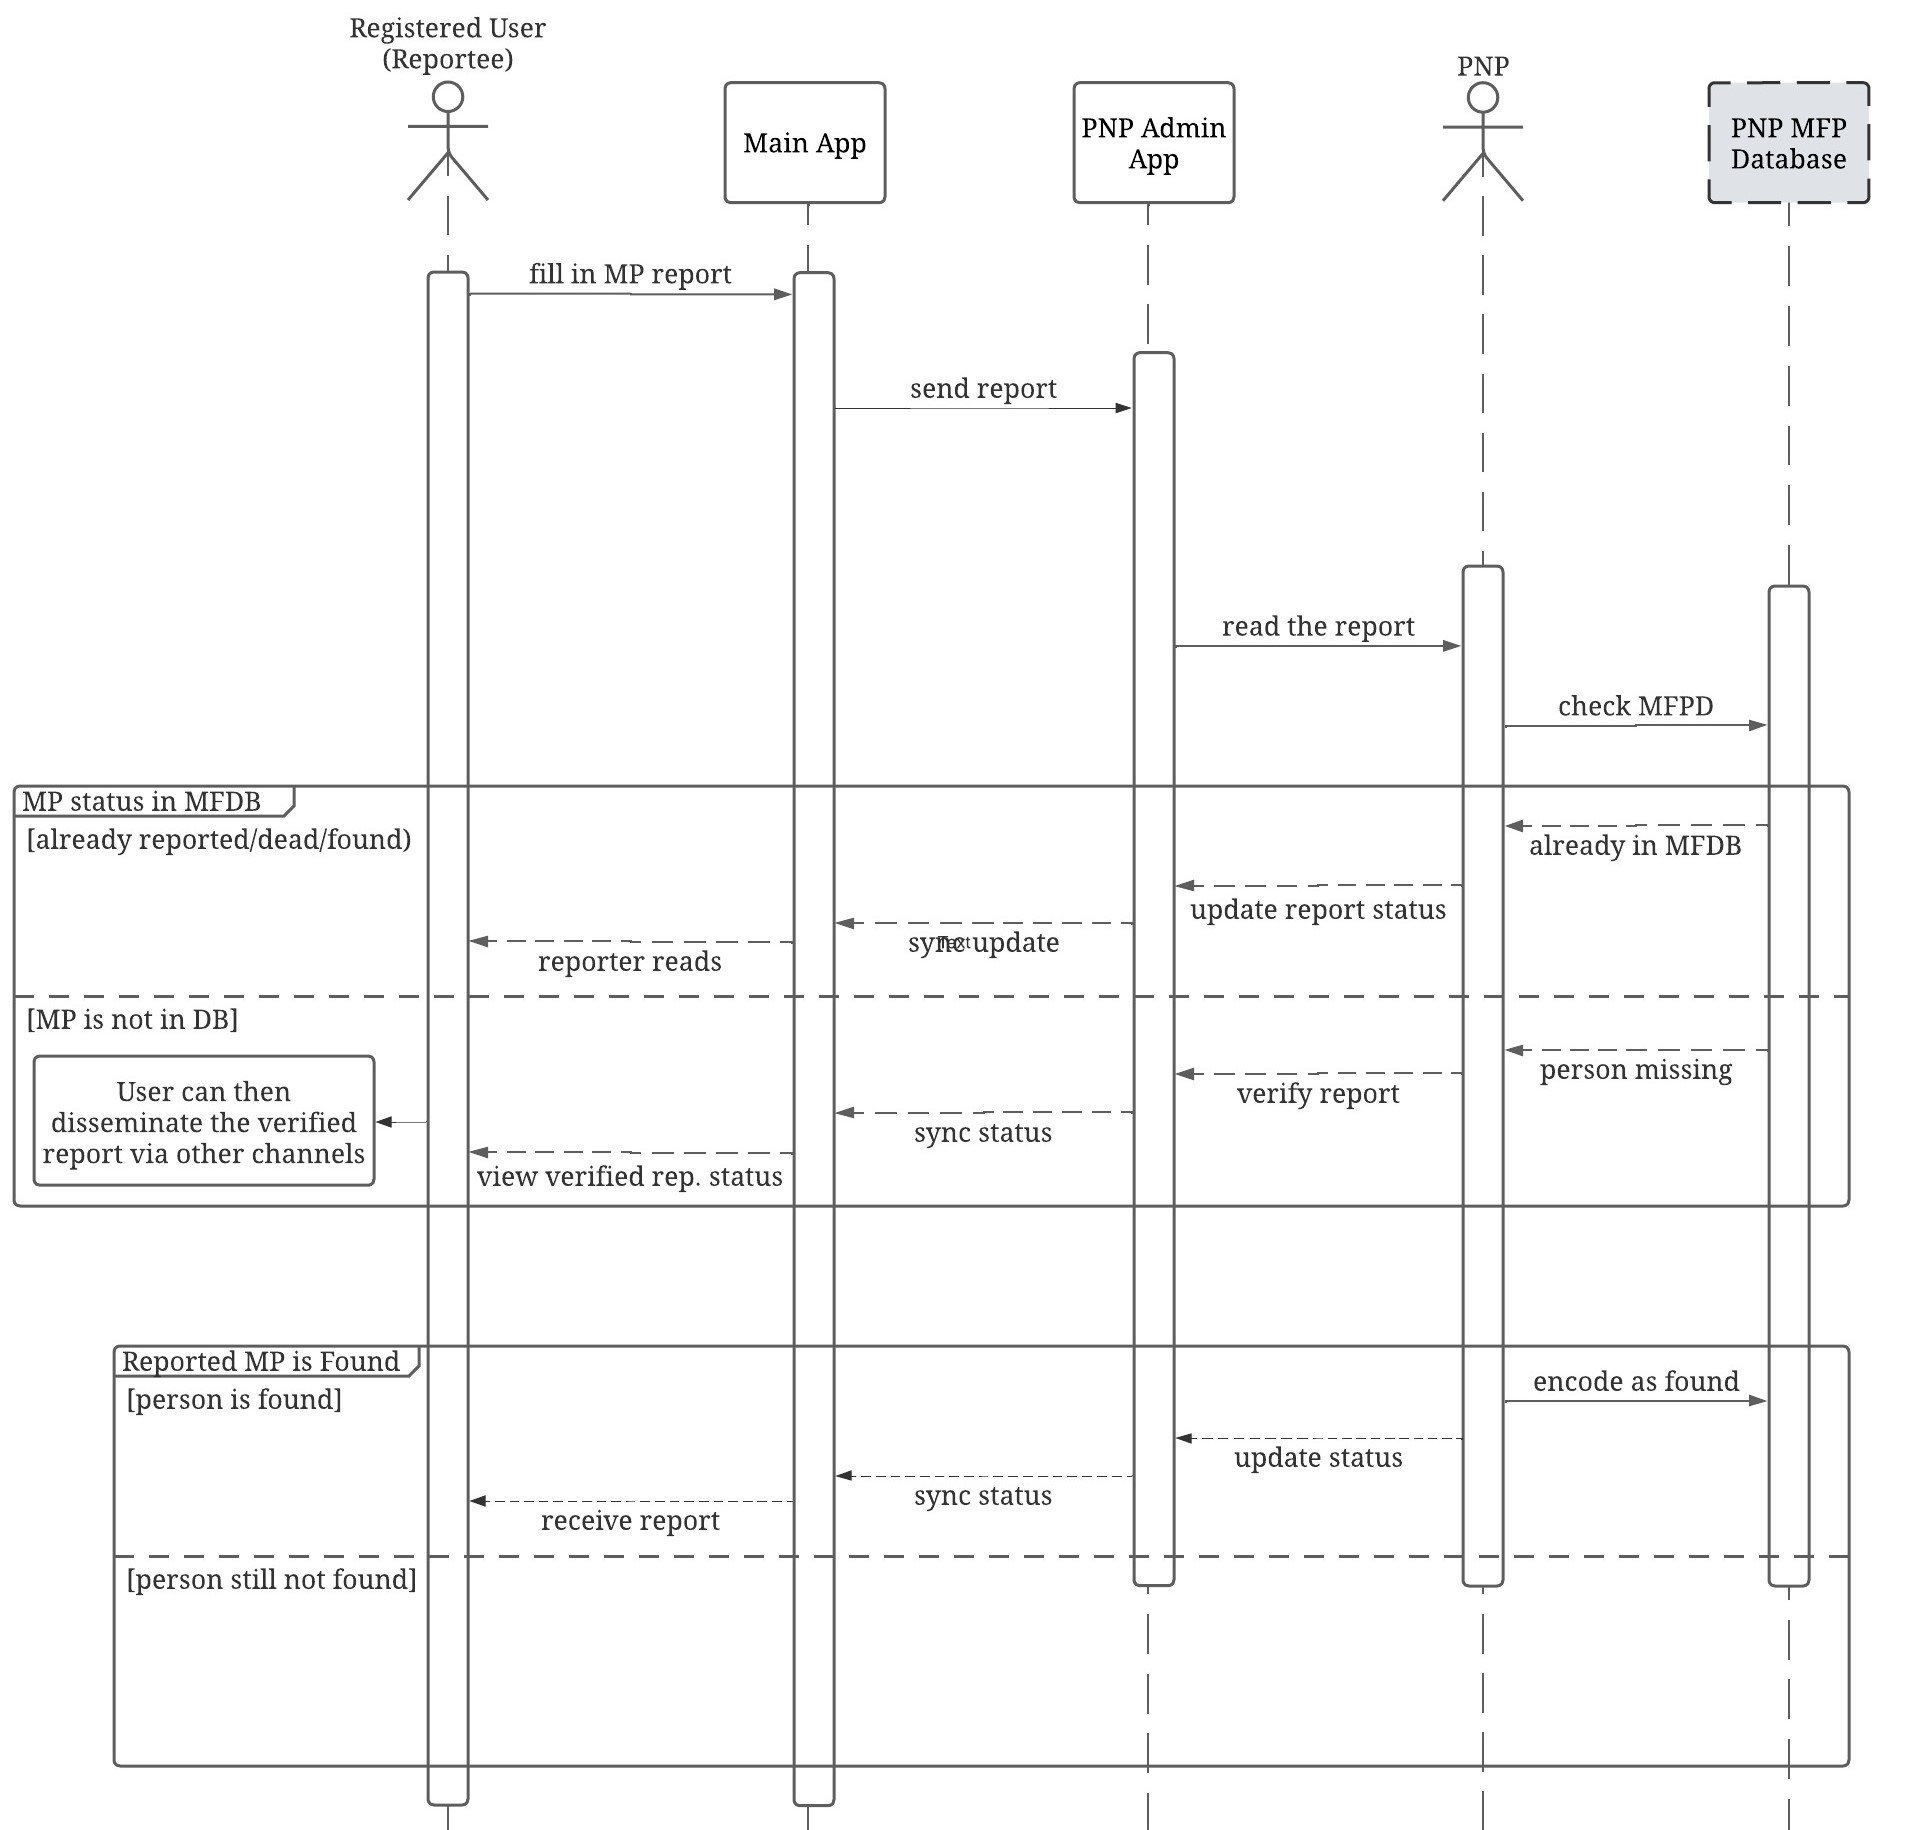
\includegraphics{figures/Chapter3/Chapt3_seqDiag_report.jpeg}
    \caption{Sequence Diagram for Reporting, Updating, and Verification of MP cases}
    \label{fig:seqDiaReport}
\end{figure}
\\\\As seen in Figure \ref{fig:seqDiaReport} sequence diagram, reporting and receiving updates is very straightforward: the user (reportee) needs to fill out the MP report form, it’s received by the PNP through their PNP Admin App interface, and if the person is indeed missing (and not yet reported, or already found, or dead), then the PNP can verify the report. If any updates are made, such as if the MP is found, it will be reflected in the user’s app soon after.

\begin{figure}[!h]
    \centering
    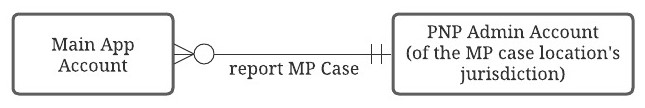
\includegraphics[width=\textwidth]{Chapter3/Chapt3_ERDiag_reporteePNP.jpeg}
    \caption{Entity Relationship Diagram of Main App Account Reporting to PNP Admin Account}
    \label{fig:ERDReportee}
\end{figure}
\\\\It’s also an important requirement that any reports made by users (reportee) are sent to the PNP Admin Account of the MP case location’s jurisdiction (and not to all PNP Admin accounts throughout the country). As seen in Figure \ref{fig:seqDiaReport} , many users should be able to submit MP case reports of a specific location to the PNP through the application, but they will only be routed to the PNP Admin Account registered for said location.

\subsubsection{Receive, Update, and Verify Reports}
The PNP Admin should be able to receive reports from users through the PNP Admin app. PNP Admin should also be able to put updates on the report (i.e. MP case already reported, MP reported is already found, MP reported is already deceased), and also verify the report to state that the MP is categorized as missing. This can also be seen in the sequence diagram in Figure \ref{fig:seqDiaReport}. 

Moreover, as mentioned in the previous requirement and as seen in Figure \ref{fig:ERDReportee} relationship diagram, the PNP Admin Account of a certain location should only receive (and be able to update/verify) MP reports from MP cases within the PNP station’s jurisdiction.

\subsubsection{Accessing PNP-Verified Reports and receiving Location-based notification for PNP-verified MP cases}

Users in a certain radius of the PNP-verified MP case receive notification about an MP case in their area. Users can tap on the notification to view details of the MP and the contact number of the reportee or PNP station in charge.

\begin{figure}[!h]
    \centering
    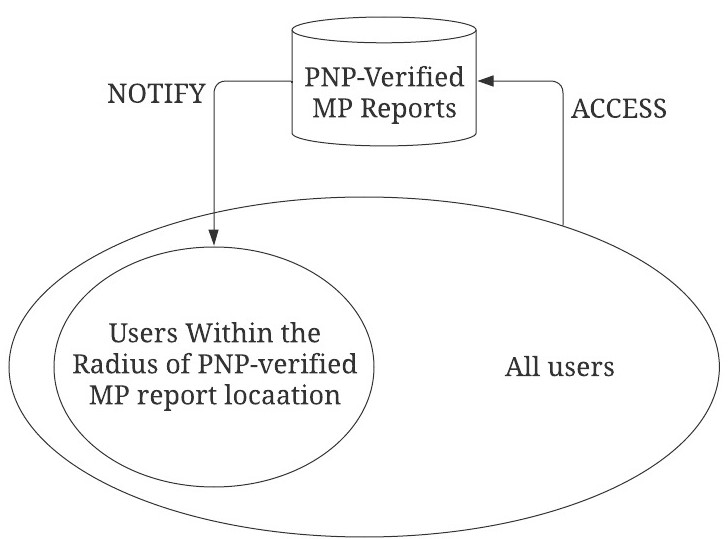
\includegraphics[width=\textwidth]{Chapter3/Chapt3_Diag_locationBasedNotif.jpeg}
    \caption{Diagram for PNP-Verified Reports Access and Notification System}
    \label{fig:diagramLocation}
\end{figure}
\\\\As seen in Figure \ref{fig:diagramLocation}, although only users in the radius of the PNP-verified MP report location will be notified, all users throughout the country will be able to view the PNP-Verified reports all over the country in order to leverage the community-based approach and cover a wider range for searching MPs. 
\\\\For ease of use, the main app will be designed wherein whenever a user checks on PNP-Verified MP Reports, the first results should be of MP cases within or near their area, and should be provided the option to filter cases by location.
\newpage
\subsubsection{User-companion binding}
Users and PARGOMs should be able to bind their accounts via the main app and companion app so that users can keep track of the companion’s location.

\begin{figure}[!h]
    \centering
    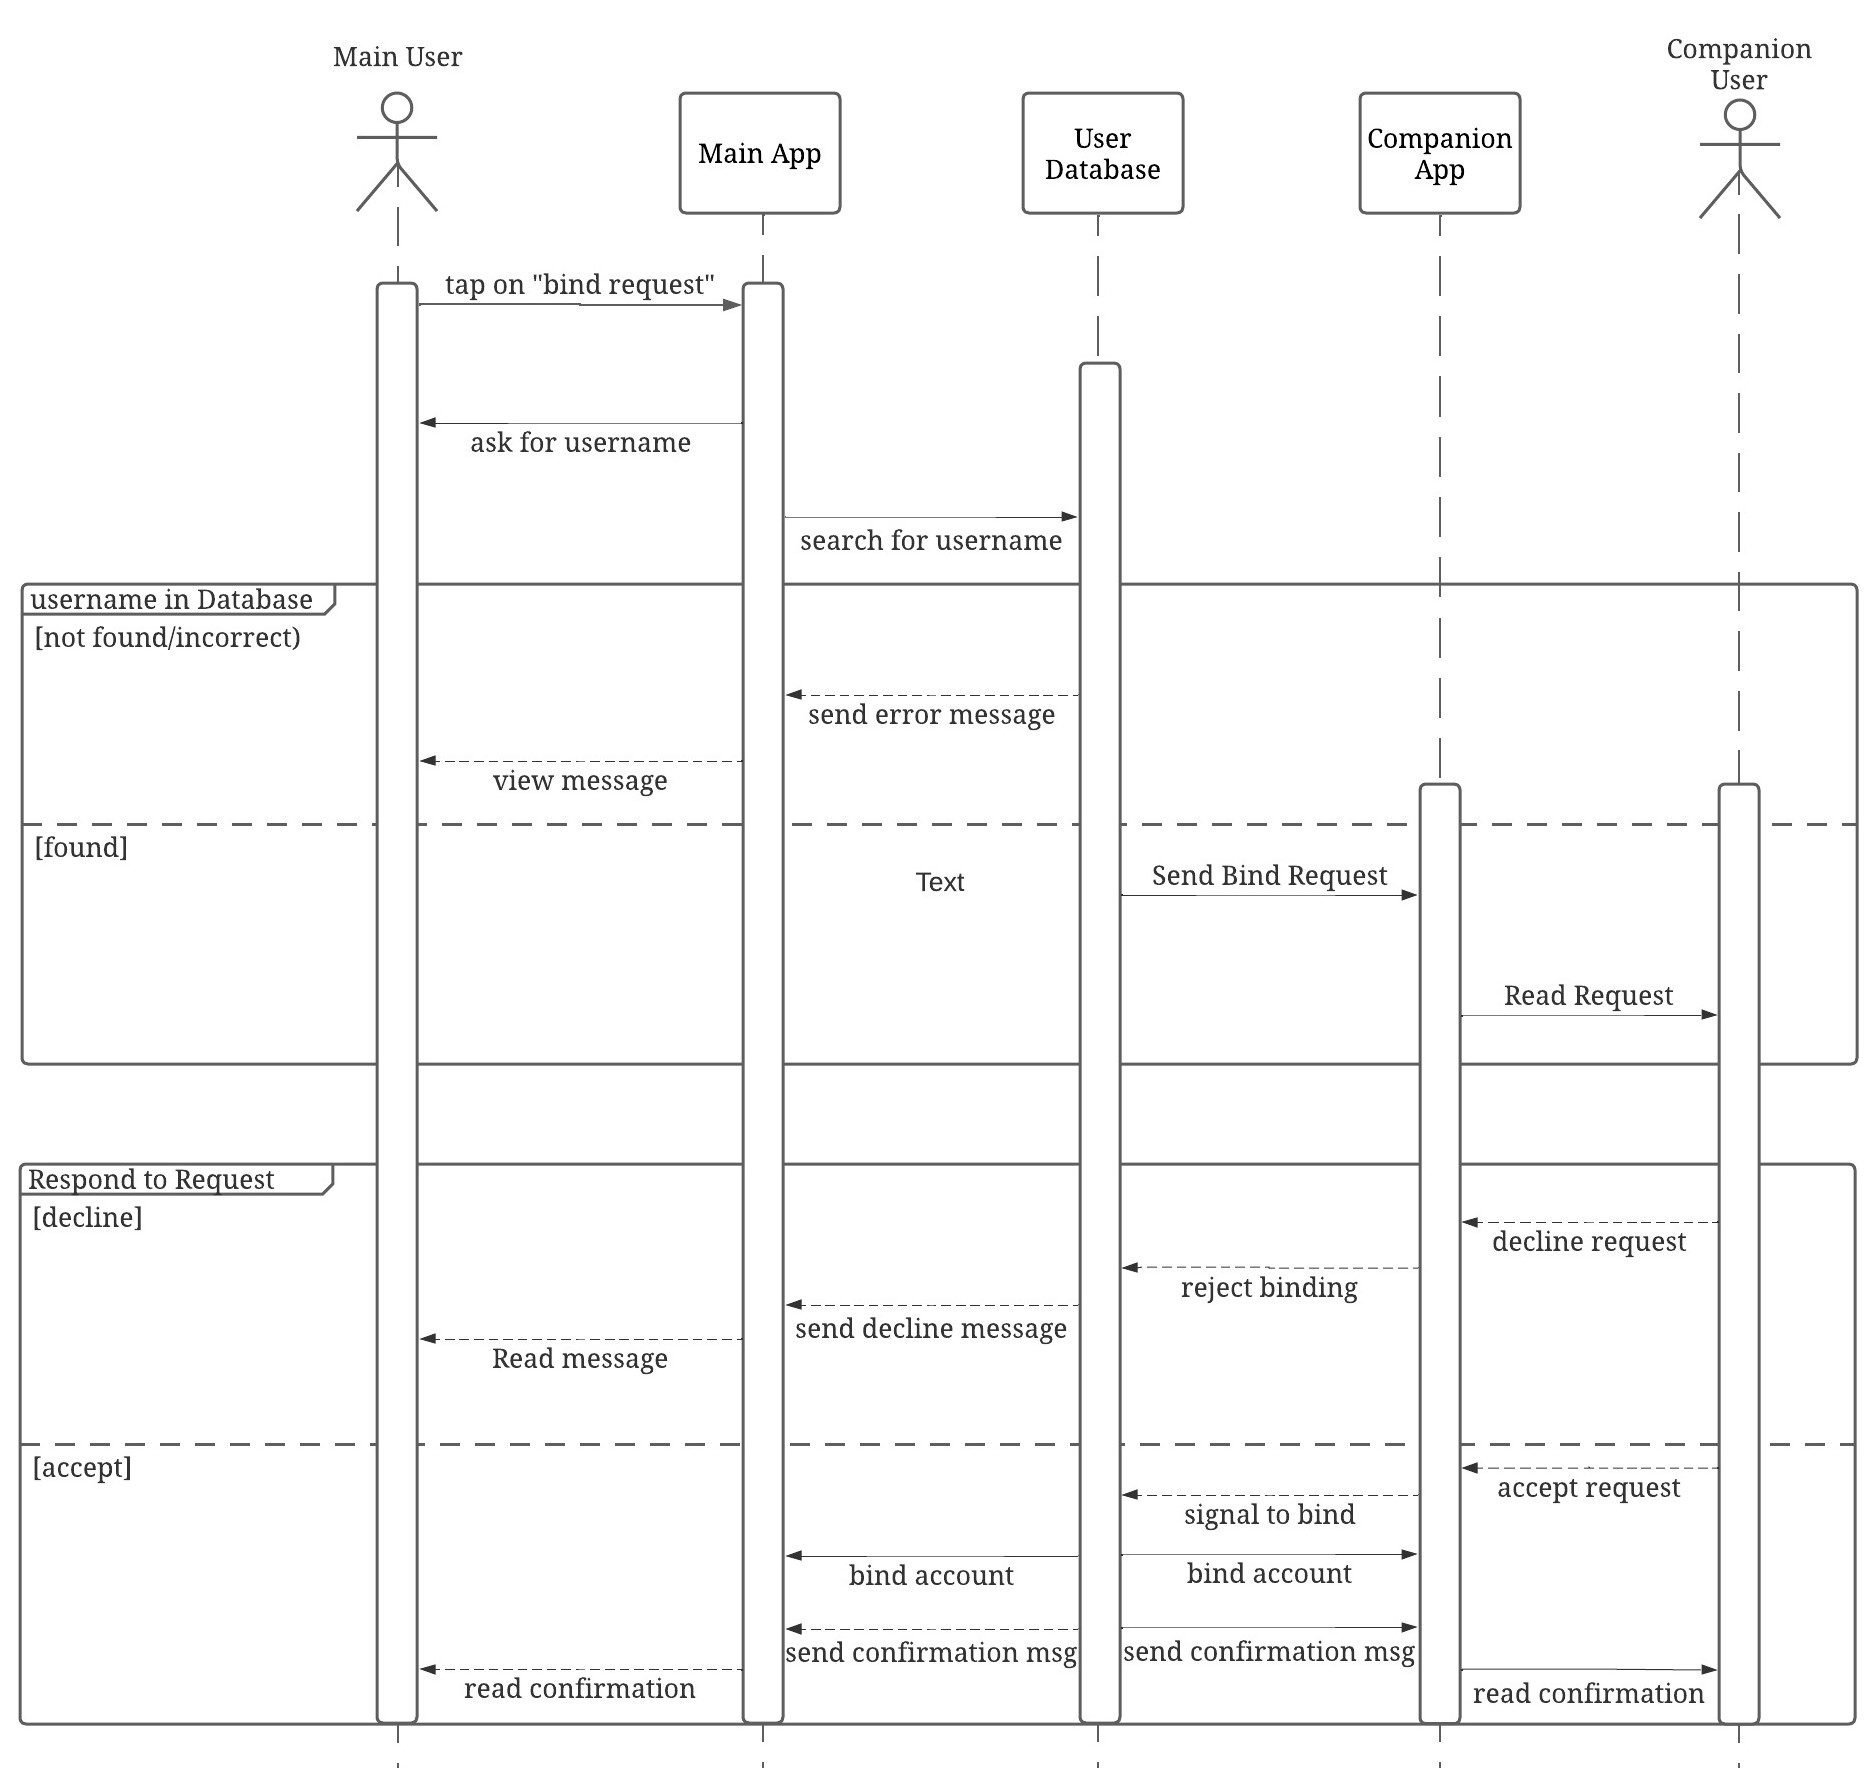
\includegraphics[width=\textwidth]{Chapter3/Chapt3_seqDiag_bind.jpeg}
    \caption{Sequence Diagram for Main-Companion Account Binding}
    \label{fig:seqDiaBind}
\end{figure}
\\\\As seen in \ref{fig:seqDiaBind} sequence diagram, the binding process is done through a simple “request-and-accept” system. The main user should be the one to initiate the binding process by entering the unique username of the companion account, and send the request. Afterwhich, the companion user should be able to either decline or accept the request for binding. Once accepted, the main and companion accounts will be binded. The purpose for this approach is to ensure that not any user could just bind their account to a companion.

\begin{figure}[!h]
    \centering
    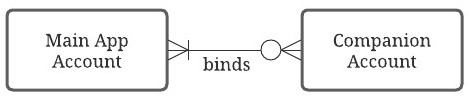
\includegraphics[width=\textwidth]{Chapter3/Chapt3_ERDiag_bind.jpeg}
    \caption{Entity Relationship Diagram of Main App Account and Companion Account}
    \label{fig:ERDBind}
\end{figure}
\\\\It’s also important that the system supports multiple account binding. As seen in Figure \ref{fig:ERDBind} relationship diagram, a companion account should always be bound to a main account for one of the main features (Find Companion) to work. Multiple main accounts can bind to multiple companion accounts (i.e. father and mother, binding their main accounts to their children’s companion accounts).

\subsubsection{User App - Find Companion Feature}
Users connected to a companion app (companion user) should be able to check the most recent location of the companion they are linked to. This is done within the main user interface. Companion users, upon connecting to a main User for the first time should be informed that the User they are linked to has access to their most recent location.

\subsubsection{Companion App - Find Me}
Companion application users should be able to use a “Find Me” button within the application in order to signal the linked User account of the companion’s current location. The “Find Me” feature should also display the nearest PNP station or help desk, and display their contact information for easy calling.